\documentclass{article}

\usepackage{hyperref}
\usepackage{amsmath}
\usepackage{graphicx}
%\usepackage{subcaption}
\usepackage{epstopdf}
\usepackage{color}

\usepackage{times}
\usepackage{bm}

% Page layout
\hoffset -0in
\voffset -1in
\oddsidemargin 0in
\textheight 9.3in
\textwidth 6.3in

\setlength{\parindent}{0pt}

\graphicspath{{figures/}}

\begin{document}
\section*{COMPUTATIONAL METHODS IN MECHANICS: Assignment 8}
Vesa-Ville Hurskainen, 28 Mar 2018\\
\href{https://github.com/VesaVilleHurskainen/cmim2018}{GitHub repository}


\section*{Introduction}
This is a report for the eighth assignment of the course \textit{Computational Methods in Mechanics}, concerning dynamic analysis. The assignment consists of five tasks, which are as follows:
\begin{enumerate}
	\setlength\itemsep{0pt}
	\item To expand the previously-made general purpose program with dynamic analysis.
	\item To allow the program to automatically select the appropriate type of analysis.
	\item To solve a four-bar linkage using the program.
	\item To test different values for Baumgarte stabilization parameters $\alpha$ and $\beta$.
	\item To compare results with an MBD package (e.g.~MSC ADAMS).
\end{enumerate}


\section*{Methods}
A diagram of the system under investigation is presented in Figure~\ref*{fig:system}. Masses of the bodies were determined to be directly proportional to length: $m_1 = m$, $m_2 = 2m$, $m_3 = m \sqrt{2}$.
\begin{figure}[htb]
	\centering
	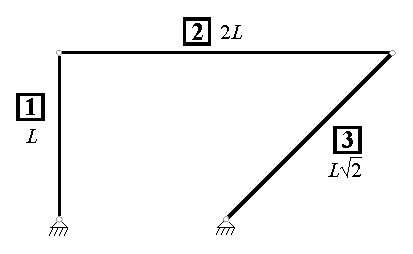
\includegraphics[width=0.4\textwidth]{system.eps}
	\caption{Diagram of the four-bar system.\label{fig:system}}
\end{figure}

To complete task 2, the function \texttt{analyse} was written. This function automatically determines the required type of analysis by checking the system's degrees of freedom and calls the appropriate function. If DOF $=$ 0, the function \texttt{run\_kinematics} is called for kinematic analysis, and if DOF $>$ 0, dynamic analysis is performed using the newly-written function \texttt{run\_dynamics}.


\section*{Results}
The system's dynamic behavior under gravity load was solved within the time span $t = 0 \dots 5$ s, with an output step size of $\Delta t = 0.01$ s. The system's physical parameters were defined as $m = 1$ kg and $L = 1$ m. Several different values for Baumgarte parameters $\alpha$ and $\beta$ were tested, and a comparison of the resulting values of constraint drift is presented in Figure~\ref*{fig:constraintdrift}.\\

Reference results were computed using MSC ADAMS, employing identical time settings. The difference between the result sets is illustrated in Figure~\ref*{fig:comparison}.

\begin{figure}[h!]
	\centering
	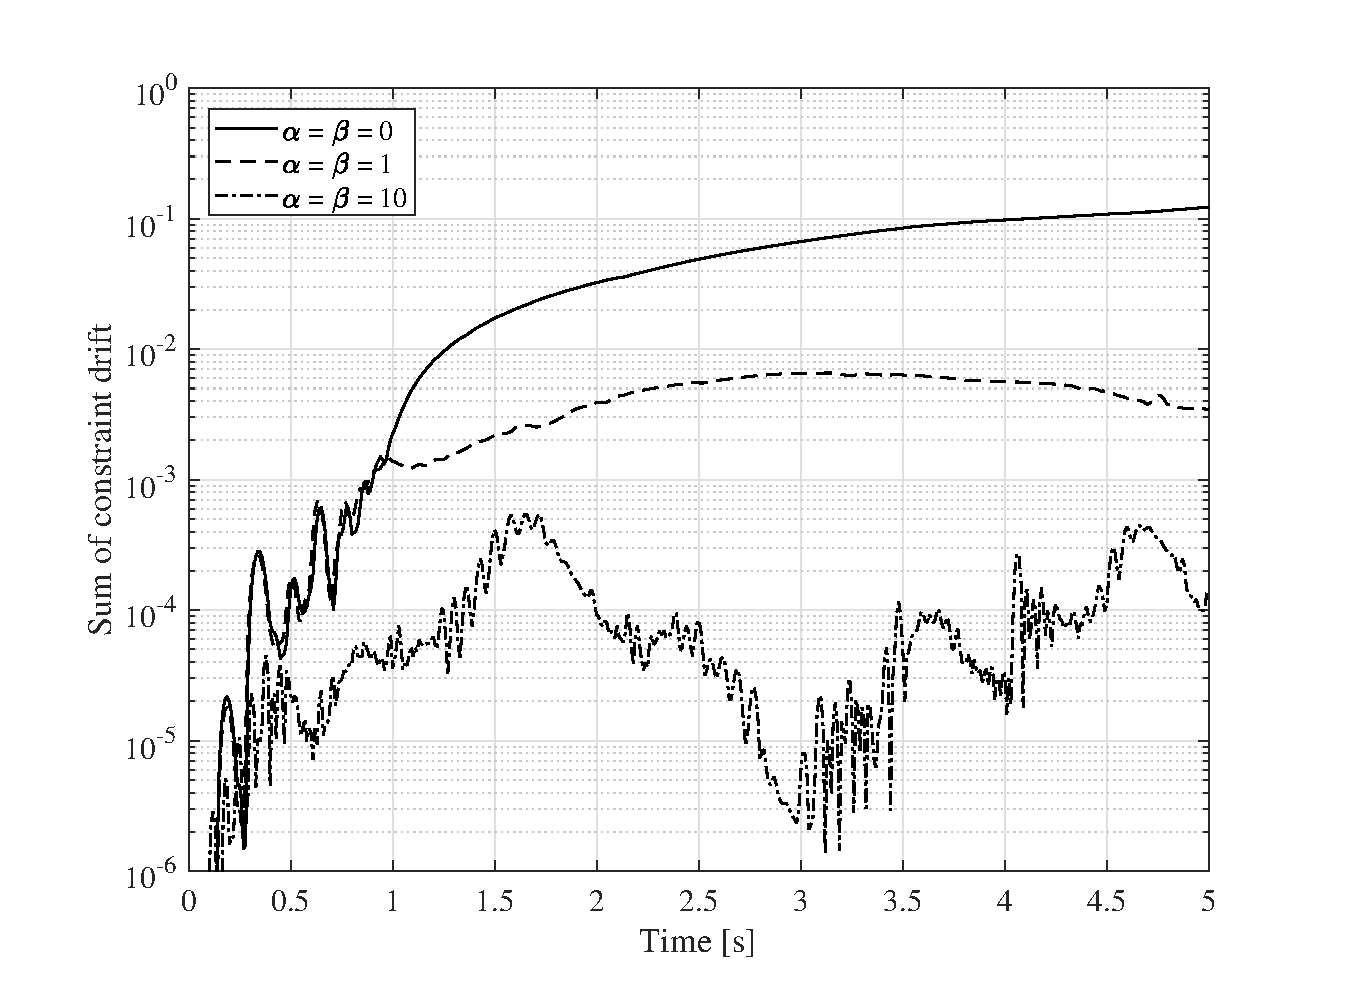
\includegraphics[width=0.8\textwidth]{constraintdrift.eps}
	\caption{Sum of constraint drift ($\sum_{i=1}^{n} |C_i| $) with different values for Baumgarte parameters.\label{fig:constraintdrift}}
\end{figure}

\begin{figure}[h!]
	\centering
	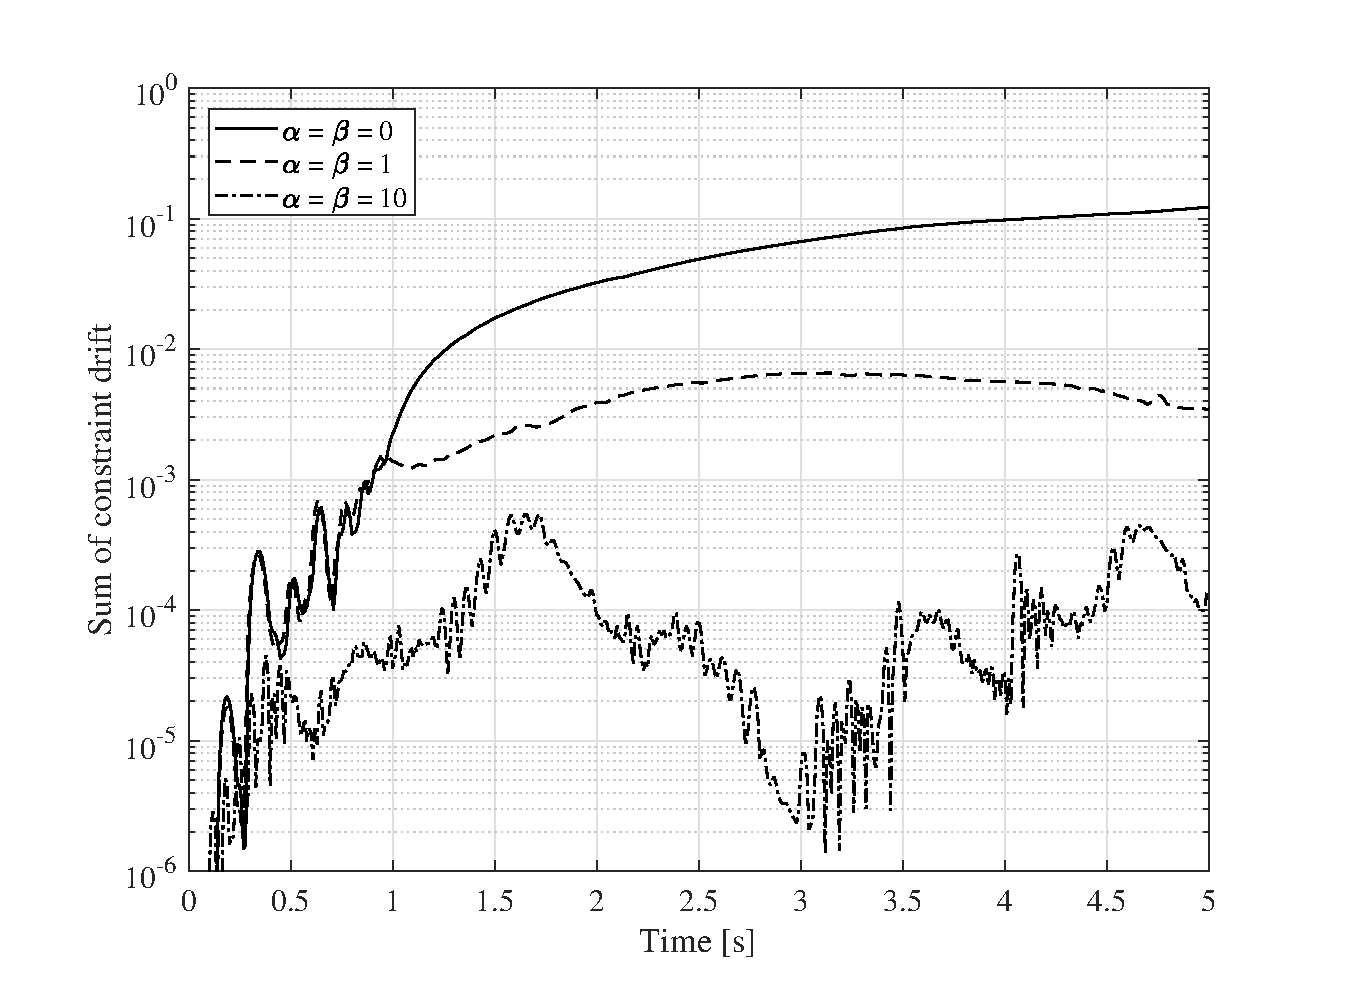
\includegraphics[width=0.8\textwidth]{constraintdrift.eps}
	\caption{Position error as function of time. Reference results computed using MSC ADAMS.\label{fig:comparison}}
\end{figure}


\section*{Analysis}
asd

\end{document}